%!TEX root=main.tex
\section{Results}

We evaluate the \mmacro{} framework, demonstrating: (1) the \mmacro{} inference engine provides a substantial speed benefit over Cholesky based inference and standard MVM-based CG inference, especially for GPU computing; (2) \mmacro{} achieves comparable or better final test error compared to Cholesky inference, even with no kernel approximations; and (3) preconditioning provides a substantial improvement in the efficiency of our approach.

\paragraph{Baseline methods.} We test \mmacro{} on three types of GPs:
1. {\bf Exact} GP models,
2. {\bf SGPR} inducing point models \cite{titsias2009variational,hensman2013gaussian},
and 3. {\bf SKI} models with Toeplitz $\K_{UU}$ and deep kernels \cite{wilson2015kernel,wilson2016deep}.
For Exact and SGPR, we compare \mmacro{} against Cholesky-based inference engines implemented in GPFlow \cite{matthews2017gpflow}.
GPFlow is presently the fastest implementation of these models with a Cholesky inference engine.
Since SKI is not intended for Cholesky inference, we compare \mmacro{} to the inference procedure of \citet{dong2017scalable}, implemented in our GPyTorch package.
This procedure differers from \mmacro{} in that it computes $\trainK^{-1} \y$ without a preconditioner and computes $\log \vert \trainK \vert$ and its derivative with the Lanczos algorithm.

\paragraph{Datasets.}
We test Exact models on five datasets from the UCI dataset repository \cite{asuncion2007uci} with up to 3500 training examples (the largest possible before all implementations exhausted GPU memory): Skillcraft, Gas, Airfoil, Autompg, and Wine.
We test SGPR on larger datasets ($n$ up to 50000): KEGG, Protein, Elevators, Kin40k, and PoleTele.
For SKI we test five of the largest UCI datasets ($n$ up to 515000): Song, Buzz, Protein, Kin40k, and KEGG.

\begin{figure}[t]
  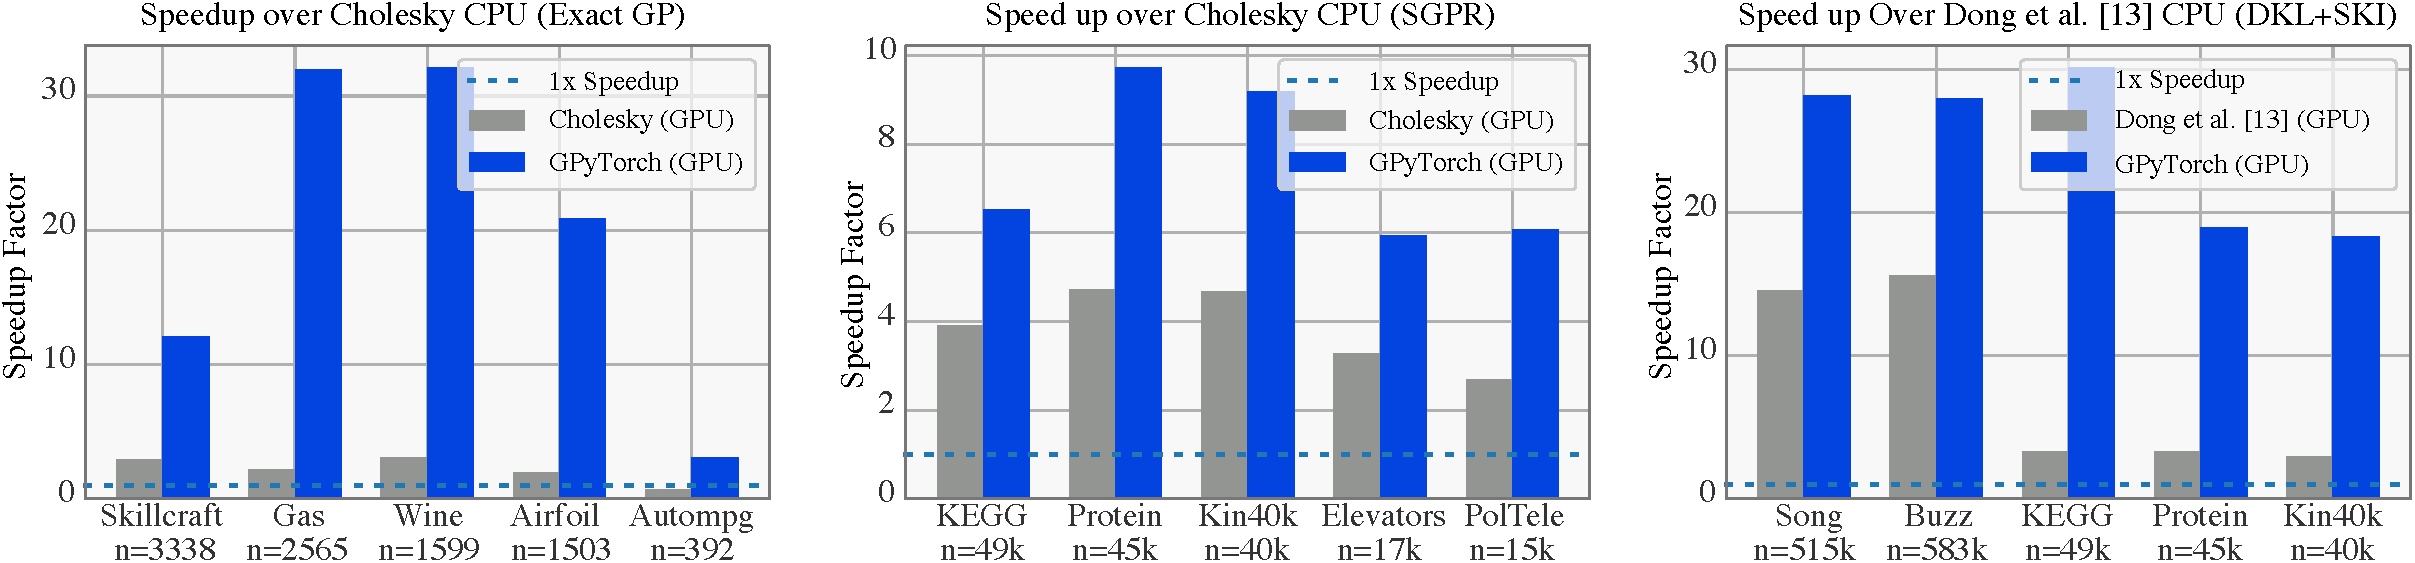
\includegraphics[width=\textwidth]{chapters/bbmm/figures/sparse_gp_results}
  \caption{
    Speedup of GPU-accelerated inference engines.
    \mmacro{} is in blue, and competing GPU methods are in gray.
    {\bf Left:} Exact GPs. {\bf Middle:} SGPR \cite{titsias2009variational,hensman2013gaussian} -- speedup over CPU Cholesky-based inference engines.
    {\bf Right:} SKI+DKL \cite{wilson2015kernel,wilson2016deep} -- speedup over CPU inference of \citet{dong2017scalable}.
  }
  \label{fig:timing_results}
\end{figure}

\paragraph{Experiment details.} All methods use the same optimizer (Adam) with identical hyperparameters.
In \mmacro{} experiments we use rank $k\!=\!5$ pivoted Cholesky preconditioners unless otherwise stated.
We use a maximum of $p\!=\!20$ iterations of CG for each solve, and
we use $t\!=\!10$ probe vectors filled with Rademacher random variables to estimate the log determinant and trace terms.
SGPR models use $300$ inducing points.
SKI models use $10,\!000$ inducing points and  the deep kernels described in \cite{wilson2016deep}.
The \mmacro{} inference engine is implemented in our GPyTorch package.
\begin{figure}[t!]
  \begin{center}
    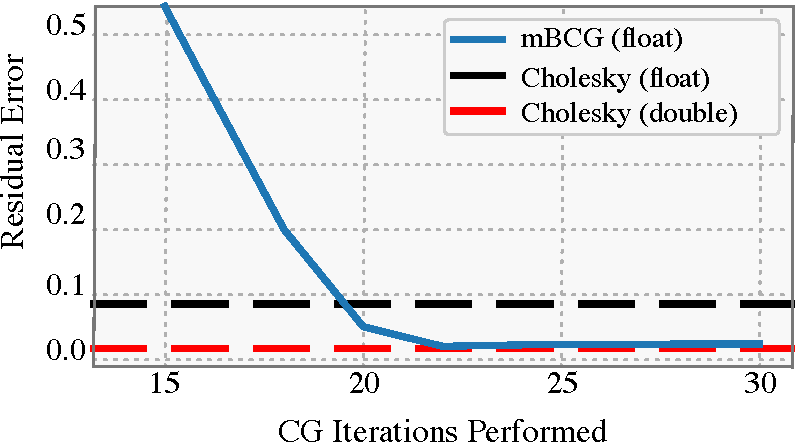
\includegraphics[width=0.48\textwidth]{chapters/bbmm/figures/cg_error}
  \end{center}
  \caption{Solve error for mBCG and Cholesky. \label{fig:cg_error}}
\end{figure}
All speed experiments are run on an Intel Xeon E5-2650 CPU and an NVIDIA Titan Xp GPU.

\label{sec:results}
%

\paragraph{Speed comparison.}
\autoref{fig:timing_results} shows the speedup obtained by GPU-accelerated \mmacro{} over the leading CPU-based inference engines (Cholesky for Exact/SGPR, \citet{dong2017scalable} for SKI).
As would be expected, GPU-accelerated \mmacro{} is faster than CPU-based inference.
On Exact and SKI, \mmacro{} is up to \emph{32 times faster} than CPU inference, and up to 10 times faster on SGPR.
The largest speedups occur on the largest datasets, since smaller datasets experience larger GPU overhead.
Notably, \mmacro{} achieves a much larger speedup than GPU accelerated Cholesky methods (Exact, SGPR), which only achieve a roughly $4\times$ speedup.
This result underscores the fact that Cholesky methods are not as well suited for GPU acceleration.
Additionally, \mmacro{} performs better than the GPU-accelerated version of \cite{dong2017scalable} on SKI.
This speedup is because \mmacro{} is able to calculate all inference terms in parallel, while \cite{dong2017scalable} computes the terms in series.
%

\begin{figure}[t]
  \centering
  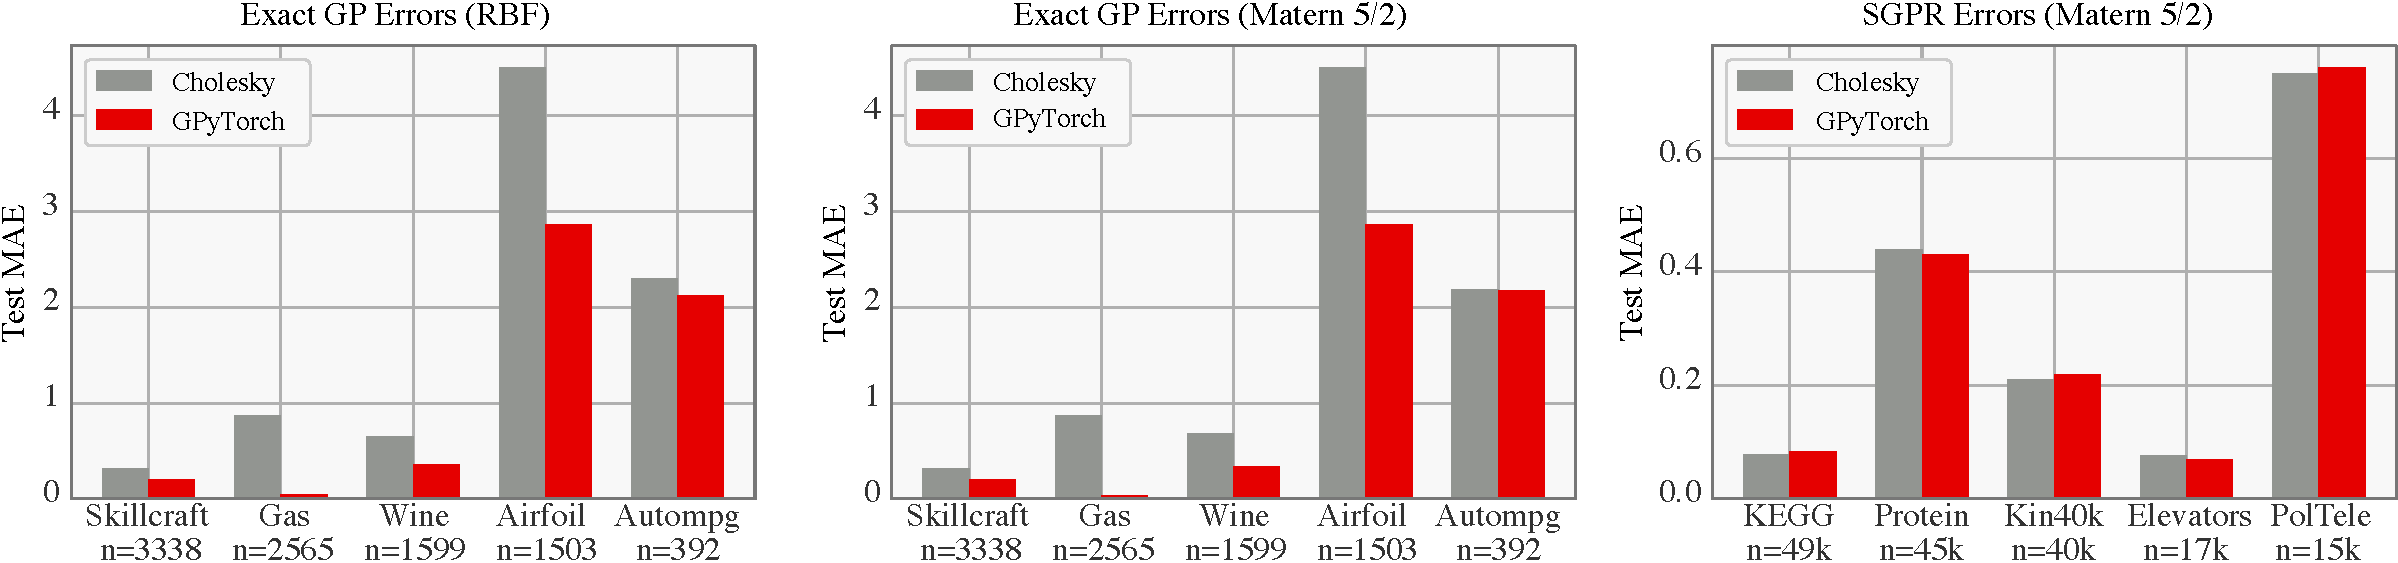
\includegraphics[width=\textwidth]{chapters/bbmm/figures/exact_gp_chol_vs_mvm}
  \caption{Comparing final Test MAE when using \mmacro{} versus Cholesky based inference. The left two plots compare errors using Exact GPs with RBF and Matern-5/2 kernels, and the final plot compares error using SGPR with a Matern-5/2 kernel on significantly larger datasets.}
  \label{fig:error_results}
\end{figure}

\paragraph{Error comparison.}
In \autoref{fig:error_results} we report test mean average error (MAE) for Exact and SGPR models.\footnote{
  SKI models are excluded from \autoref{fig:error_results}.
  This is because the \mmacro{} inference engine and the inference engine of \citet{dong2017scalable} return identical outputs (see \autoref{app:mod_cg}) even though \mmacro{} is faster.
}
We demonstrate results using both the RBF kernel and a Matern-5/2 kernel.
Across all datasets, our method is at least as accurate in terms of final test MAE.
On a few datasets (e.g. Gas, Airfoil, and Wine with Exact GPs) \mmacro{} even improves final test error.
CG has a regularizing effects which may improve methods involving the exact kernel over the Cholesky decomposition, where numerical issues resulting from extremely small eigenvalues of the kernel matrix are ignored.
For example, Cholesky methods frequently add noise (or ``jitter'') to the diagonal of the kernel matrix for numerical stability.
It is possible to reduce the numerical instabilities with double precision (see \autoref{fig:cg_error}); however, this requires an increased amount of computation.
\mmacro{} on the other hand avoids adding this noise, without requiring double precision.

\begin{figure}[t]
  \centering
  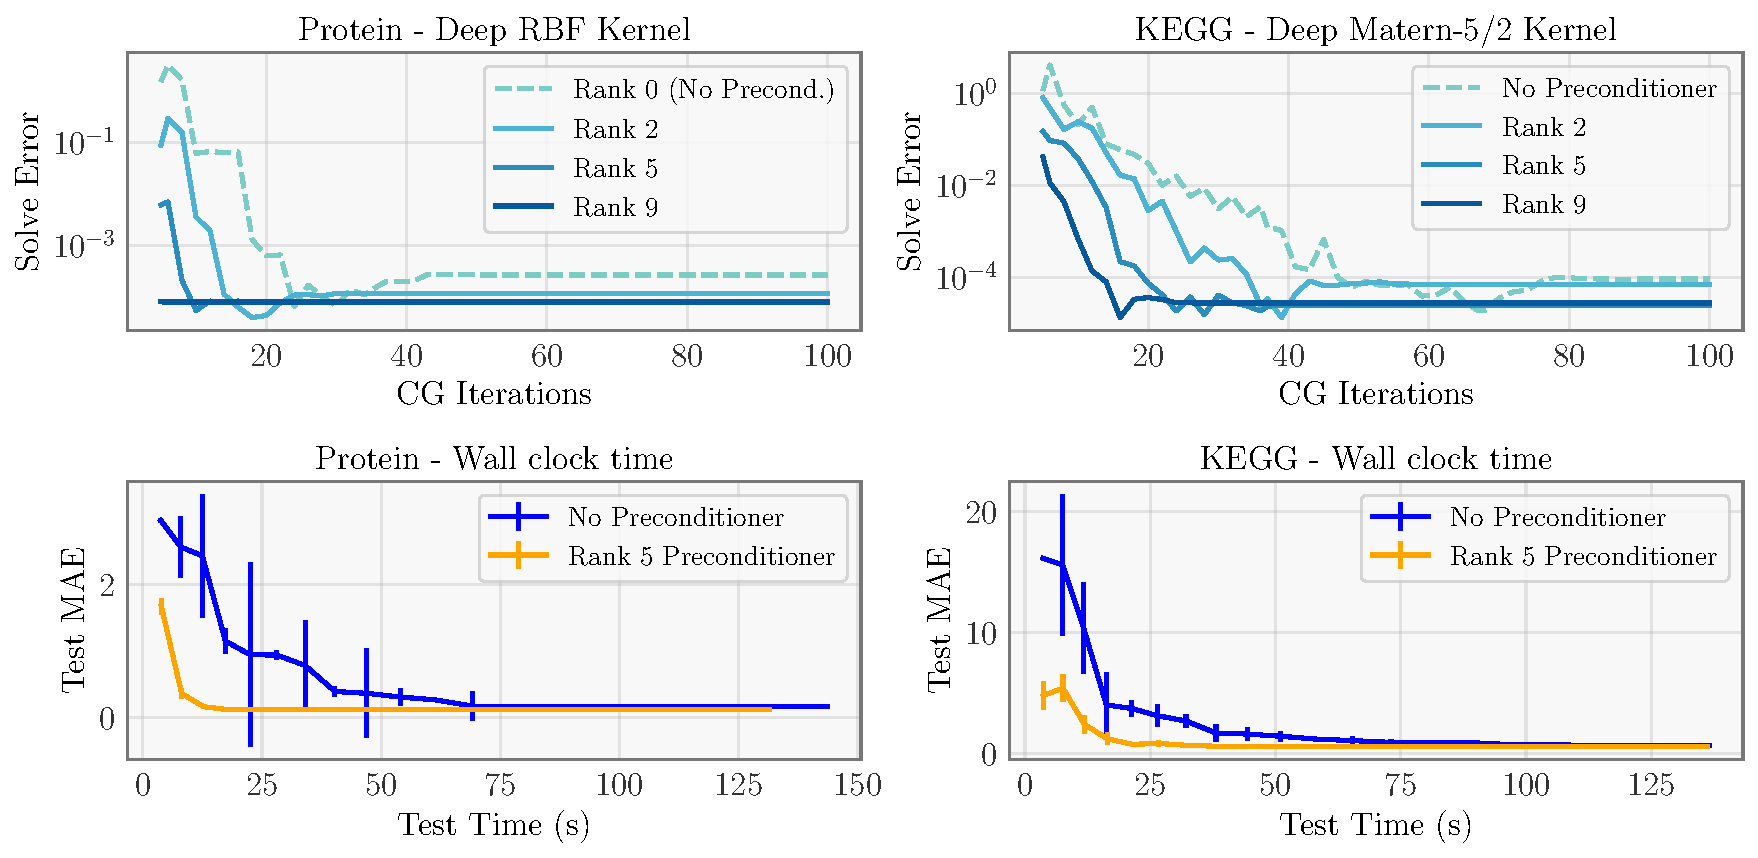
\includegraphics[width=\textwidth]{chapters/bbmm/figures/precond_solves}
  \caption{
    The effect of preconditioning on solve errors $\Vert K\x^{*} - \by \Vert / \Vert \by \Vert$ achieved by linear conjugate gradients using no preconditioner versus rank 2, 5, and 9 pivoted Cholesky preconditioners on 2 UCI benchmark datasets using deep RBF and deep Matern kernels.
    The hyperparameters of $K$ were learned by maximizing the marginal log likelihood on each dataset.
  }
  \label{fig:precond_results}
\end{figure}

\paragraph{Preconditioning.}
To demonstrate the effectiveness of preconditioning at accelerating the convergence of conjugate gradients, we first train a deep RBF kernel model on two datasets, Protein and KEGG, and evaluate the solve error of performing $\trainK^{-1}\y$ in terms of the relative residual $\Vert \trainK\bu - \y \Vert / \Vert \y \Vert$ as a function of the number of CG iterations performed.
We look at this error when using no preconditioner, as well as a rank 2, 5, and 9 preconditioner.
To demonstrate that the preconditioner is not restricted to use with an RBF kernel, we evaluate using a deep RBF kernel on Protein and a deep Matern-5/2 kernel on KEGG.
The results are in the top of \autoref{fig:precond_results}.
As expected based on our theoretical intuitions for this preconditioner, increasing the rank of the preconditioner substantially reduces the number of CG iterations required to achieve convergence.

In the bottom of \autoref{fig:precond_results}, we confirm that these more accurate solves indeed have an effect on the final test MAE.
We plot, as a function of the total wallclock time required to compute predictions, the test MAE resulting from using no preconditioner and from using a rank 5 preconditioner.
The wallclock time is varied by changing the number of CG iterations used to compute the predictive mean.
We observe that, because such a low rank preconditioner is sufficient, using preconditioning results in significantly more accurate solves while having virtually no impact on the running time of each CG iteration.
Consequentially, we recommend always using the pivoted Cholesky preconditioner with BBMM since it has virtually no wall-clock overhead and rapidly accelerates convergence.
